%%%%%%%%%%%%%%%%%%%%%%%%%%%%%%%%%%%%%%%%%%  不使用 authblk 包制作标题  %%%%%%%%%%%%%%%%%%%%%%%%%%%%%%%%%%%%%%%%%%%%%%
%-------------------------------PPT Title-------------------------------------
\title{化学-化工知识图谱的建设与应用}
%-----------------------------------------------------------------------------
%----------------------------Author & Date------------------------------------

%\author[\textrm{Jun\_Jiang}]{姜\;\;骏\inst{}} %[]{} (optional, use only with lots of authors)
%% - Give the names in the same order as the appear in the paper.
%% - Use the \inst{?} command only if the authors have different
%%   affiliation.
\institute[BCC]{\inst{}%
%\institute[Gain~Strong]{\inst{}%
\vskip -20pt 北京市计算中心}
%\vskip -20pt {\large 格致斯创~科技}}
\date[\today] % (optional, should be abbreviation of conference name)
{%	{\fontsize{6.2pt}{4.2pt}\selectfont{\textcolor{blue}{E-mail:~}\url{jiangjun@bcc.ac.cn}}}
\vskip 45 pt {\fontsize{8.2pt}{6.2pt}\selectfont{%清华大学\;\;物理系% 报告地点
	\vskip 5 pt \textrm{2023.10.14}}}
}

%% - Either use conference name or its abbreviation
%% - Not really information to the audience, more for people (including
%%   yourself) who are reading the slides onlin%%   yourself) who are reading the slides onlin%%   yourself) who are reading the slides onlineee
%%%%%%%%%%%%%%%%%%%%%%%%%%%%%%%%%%%%%%%%%%%%%%%%%%%%%%%%%%%%%%%%%%%%%%%%%%%%%%%%%%%%%%%%%%%%%%%%%%%%%%%%%%%%%%%%%%%%%

\subject{}
% This is only inserted into the PDF information catalog. Can be left
% out.
%\maketitle
\frame
{
%	\frametitle{\fontsize{9.5pt}{5.2pt}\selectfont{\textcolor{orange}{“高通量并发式材料计算算法与软件”年度检查}}}
\titlepage
}
%-----------------------------------------------------------------------------

%------------------------------------------------------------------------------列出全文 outline ---------------------------------------------------------------------------------
%\section*{}
%\frame[allowframebreaks]
%{
%  \frametitle{Outline}
%%  \frametitle{\textcolor{mycolor}{\secname}}
%  \tableofcontents%[current,currentsection,currentsubsection]
%}
%%在每个section之前列出全部Outline
%%类似的在每个subsection之前列出全部Outline是\AtBeginSubsection[]
%\AtBeginSection[]
%{
%  \frame<handout:0>%[allowframebreaks]
%  {
%    \frametitle{Outline}
%%全部Outline中,本部分加亮
%    \tableofcontents[current,currentsection]
%  }
%}

%-----------------------------------------------PPT main Body------------------------------------------------------------------------------------
\small
%\section{\rm{VASP~}软件中\rm{PAW~}计算的实现}
%\frame
%
%	\frametitle{\textrm{VASP}计算的特色}
%	相比于与普通的第一原理计算软件,\textrm{VASP}很好地平衡了计算效率和精度的问题,总的来说,\textrm{VASP}主要通过这几个特色保证了计算的高效能
%	\begin{itemize}
%	     \item 迭代与优化算法的多样性\\
%		     本质上电荷密度迭代 \textrm{\&\&} 体系总能量优化是相同的优化问题,采用了类似的算法\upcite{CMS6-15_1996,PRB54-11169_1996}:\\
%			\textcolor{blue}{\textrm{Pseudo-Newton、Conjugate-Gradient、Broyden~mix、damping-factor、RMM-DIIS}}
%	     \item 尽可能采用局域基(原子轨道基)函数:~\\
%		     \textcolor{blue}{\textrm{LREAL}}=\textcolor{red}{\textrm{.TRUE.}}\\
%			优化的投影函数也尽可能在实空间表示
%	     \item \textrm{PAW}原子数据集:\textcolor{blue}{优异的赝势}\upcite{PRB59-1758_1999}
%	\end{itemize}
%}
\frame
{
	\frametitle{数据、信息与知识}
\begin{figure}[h!]
\centering
\vskip -10pt
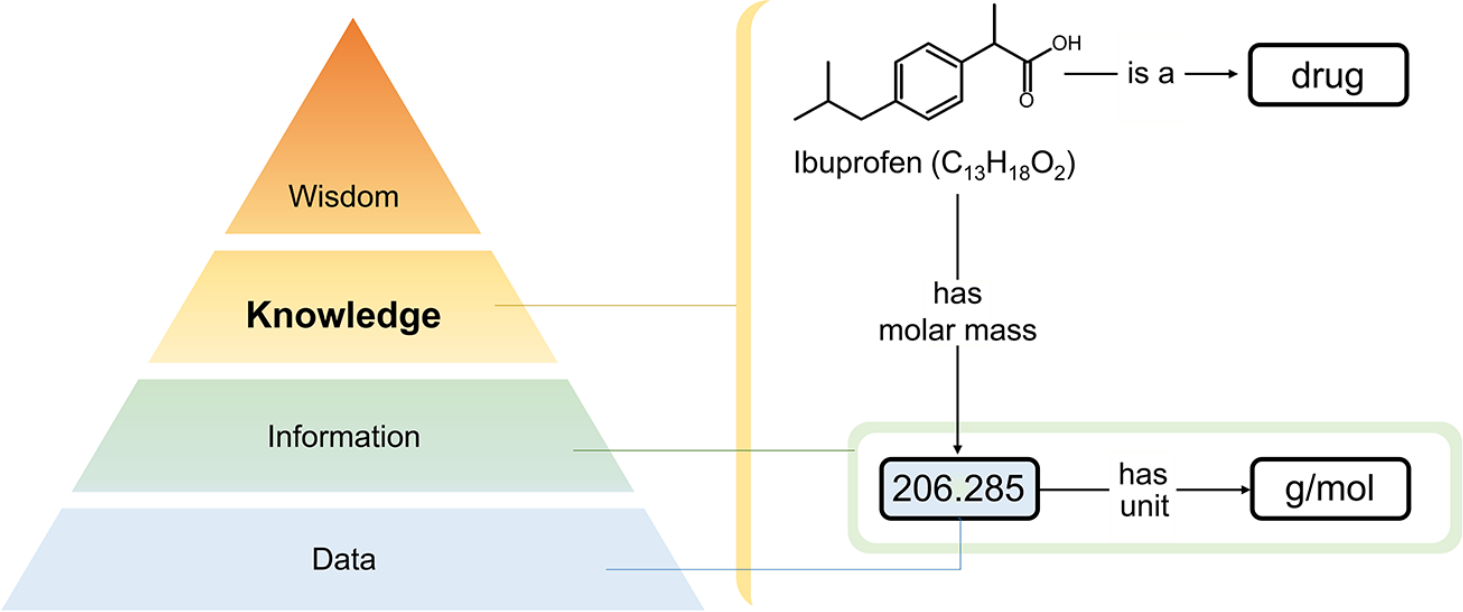
\includegraphics[height=1.75in,width=4.00in,viewport=0 0 1490 615,clip]{DIKW_pyramid-illustrating-data_information-knowledge.png}
\caption{\tiny\textrm{Schematic representation of the DIKW pyramid illustrating the meaning of data, inforamation, and knowledge in the chemical context.\cite{ACR56-128_2023}}}%(与文献\cite{EPJB33-47_2003}图1对比)
\label{Fig:Knowledge-based_system}
\end{figure}
\textcolor{magenta}{知识}\textrm{(Knowledge)}:\\
哲学学科——诸如认知论和方法论——中的核心主题
}

\section{知识图谱基础知识}
\frame
{
	\frametitle{知识图谱}
	\textcolor{blue}{知识图谱}~\textrm{(Knowledge Graph)}:
	\begin{itemize}
		\item 一种用于组织、表示和存储知识的图形化数据结构形式
		\item \textcolor{purple}{目的}:~使计算机能够更好地认知、理解和推理知识\\
			仿照人类对于知识的认知、理解方式\\
			将实体\textrm{(Entities)}、关系\textrm{(Relationship)}和属性\textrm{(Attributes)}以图形的形式呈现出来,
		\item \textcolor{purple}{技术底层}:~基于语义网\textrm{(Semantic Web)}技术\\
			以\textrm{Web}数据的内容(即语义)为核心,用机器能够理解和处理的方式链接起来的海量分布式数据库
	\end{itemize}
%	知识图谱得益于\textrm{Web}的发展(主要的是数据层面),有着来源于\textrm{KR}、\textrm{NLP}、\textrm{Web}、\textrm{AI}多个方面的基因
\begin{figure}[h!]
\centering
\vskip -8pt
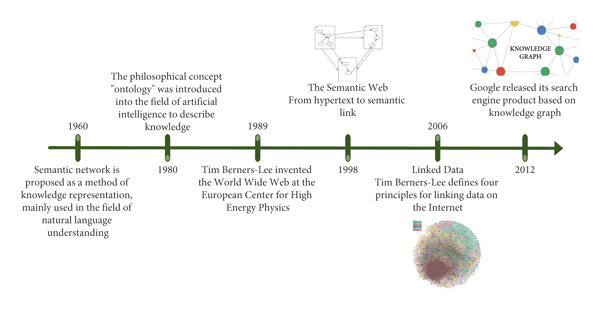
\includegraphics[height=1.00in,width=2.50in,viewport=0 0 160 75,clip]{Development-history-of-the-knowledge-graph.jpg}
\caption{\tiny\textrm{Schematic representation of the development history of the Knowledge Graph.}}%(与文献\cite{EPJB33-47_2003}图1对比)
\label{Fig:Knowledge-history}
\end{figure}
}

\frame
{
	\frametitle{知识图谱的要素}
知识图谱以图形结构的方式,通常使用节点(实体)和连线/边(关系)的形式表示知识\\
这种结构使得知识点之间的关联关系更加清晰和可视化

主要的关键词为:
\begin{itemize}
	\item 实体\textrm{(Entities)}:~知识图谱中的实体是指具体的事物、概念、人物、地点等,每个实体都有一个唯一的标识符\\
		例如,在化学知识图谱中,分子、合成体、密度等都是实体。
	\item 关系\textrm{(Relationships)}:~实体之间的关系表示不同实体之间的连接或互动。这些关系可以是有向的或无向的,用于描述实体之间的各种联系\\
		如” 具有”、” 属于”、”值为” 等。
	\item 属性\textrm{(Attributes)}:~实体可以有一些描述性的属性,这些属性是与实体相关的额外信息\\
		例如,分子(实体)的属性,包括分子量、化合价、密度等。
\end{itemize}
}

\frame
{
	\frametitle{资源的描述}
\begin{figure}[h!]
\centering
\vskip -8pt
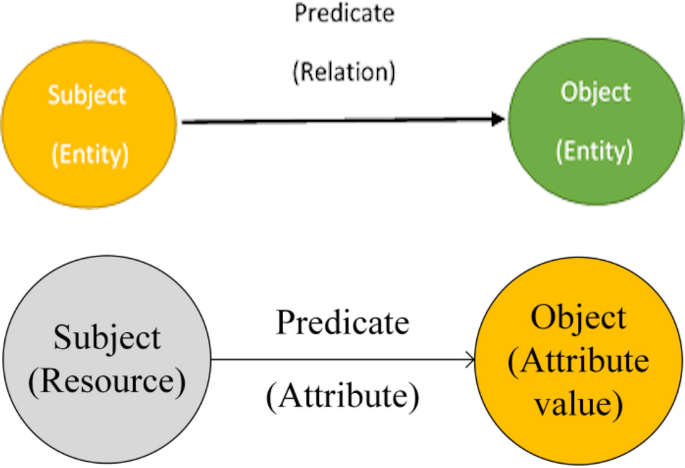
\includegraphics[height=2.35in,width=3.50in,viewport=0 0 690 470,clip]{KG-Entity-relation_0.png}
\caption{\tiny\textrm{Schematic representation of the relationship between entites.}}%(与文献\cite{EPJB33-47_2003}图1对比)
\label{Fig:KG-Entity-relations}
\end{figure}
}

\frame
{
	\frametitle{领域知识的描述:~\textrm{Ontology}}
	\textrm{Ontology}:~用于描述学科领域知识的通用概念模型,模型包含了学科内基本术语-术语间关系,是领域内概念的集合,\textcolor{blue}{属于群体概念}
	\begin{itemize}
		\item \textrm{Ontology}:~是哲学概念,哲学中关系的是客观存在的抽象本质
		\item 在语义学层次上,\textrm{Onlogy}是\textcolor{red}{共享概念模型的格式化规范说明}
	\begin{itemize}
		\item 共享\textrm{(Share)}:~知识必须是共同认可的
		\item 概念化\textrm{(Conceptualization)}:~对事物的描述构成一组概念
		\item 明确性\textrm{(Explicit)}:~每个术语、属性都有明确定义
		\item 格式化\textrm{(Format)}:~可以被计算机处理
	\end{itemize}
\item \textrm{Ontology}的描述语言主要有\textrm{RDF}、\textrm{RDFS}和\textrm{OWL}
	\begin{itemize}
		\item \textrm{RDF}:~用于描述\textrm{Web}上的资源\\
			用\textrm{Web}标识符来标记资源(主语),用属性(谓语)和属性值(宾语)来描述资源
		\item \textrm{RDFS}:~在\textrm{RDF}基础上扩展而成,更形象地表达知识
		\item \textrm{OWL}:~保持\textrm{RDF}、\textrm{RDFS}的兼容性,用于\textrm{ontology}的语义描述
	\end{itemize}
	\end{itemize}
}

\frame
{
	\frametitle{\textrm{RDF}举例:~分子与合成体的描述}
\begin{figure}[h!]
\centering
\vskip -8pt
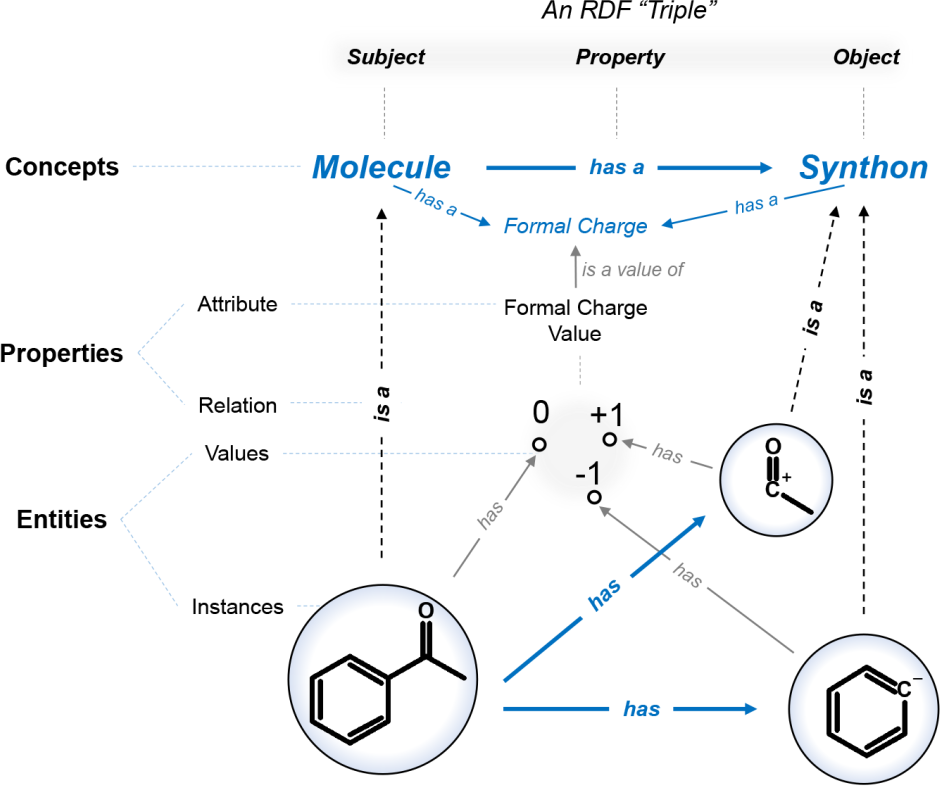
\includegraphics[height=2.60in,width=3.45in,viewport=0 0 950 790,clip]{Mapping-the-relationship-between-molecule-and-synthon.png}
\caption{\tiny\textrm{Mapping the relationship molecule (chemical) and synthon (abstract) concepts and illustrating them with instrances. cite from\cite{ACR56-128_2023}}}%(与文献\cite{EPJB33-47_2003}图1对比)
\label{Fig:Mapping-relationship-molecule-synthon}
\end{figure}
}

\section{化学-化工知识图谱}
\frame
{
	\frametitle{化学-化工知识图谱的组成}
\begin{figure}[h!]
\centering
\vskip -8pt
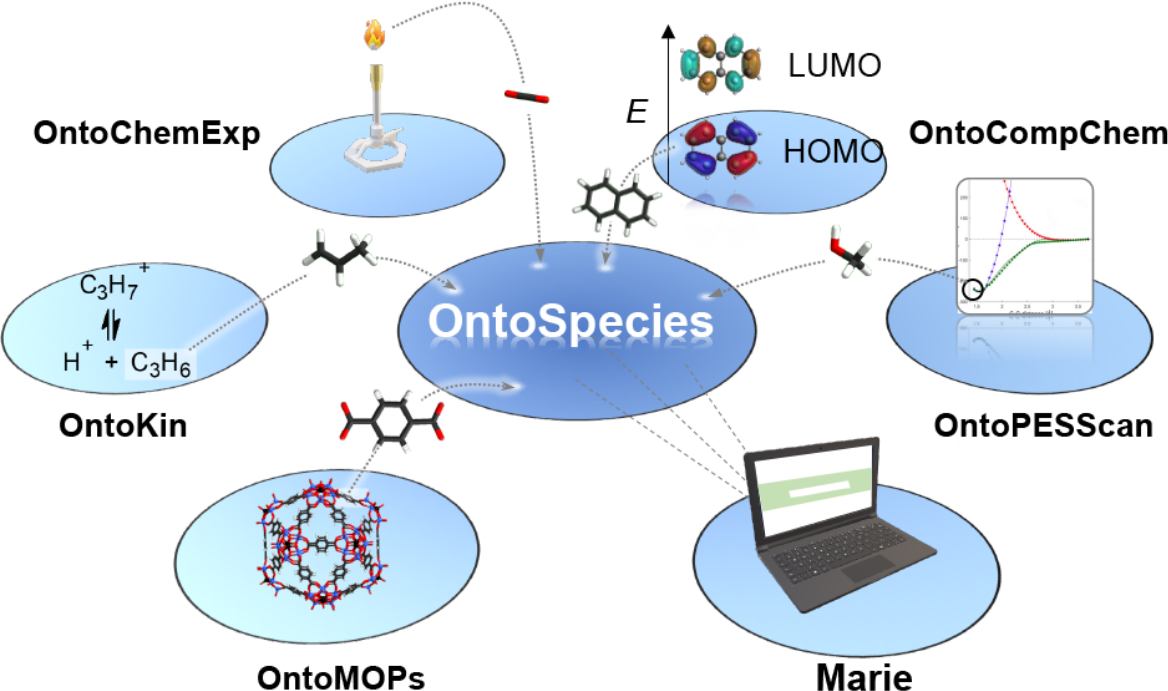
\includegraphics[height=2.45in,width=4.05in,viewport=0 0 1170 700,clip]{Connection-of-OntoSpecies-to-segments-of-KG.png}
\caption{\tiny\textrm{Connection of OntoSpecies to other segments of TWA KG. cite from\cite{ACR56-128_2023}}}%(与文献\cite{EPJB33-47_2003}图1对比)
\label{Fig:OntoSpecies-to-segments-TWA}
\end{figure}
}

\frame
{
	\frametitle{化学-化工知识图谱}
	化学-化工知识图谱:~以化学物种(元素、化合物)为核心的\textcolor{cyan}{多个知识的\textrm{Ontology}组成}
	\begin{itemize}
		\item \textrm{OntoSpecites}:~主要纪录化学物种的知识,包括分子式、电荷、分子量和自旋多重度等
		\item \textrm{OntoKin}:~表示反应机理的知识,纪录反应物、产物和反应过程的信息
		\item \textrm{OntoCompChem}:~表示计算化学的信息的知识,计算信息的描述包括
			\begin{itemize}
				\item 计算对象:~单点计算、结构优化和频率计算
				\item 计算使用的软件,{\fontsize{7.2pt}{5.2pt}\selectfont{如\textrm{Gaussian~16}}}
				\item 计算中使用的方法,包括泛函和基组{\fontsize{7.2pt}{5.2pt}\selectfont{~如\textrm{B3LYP,~6-31G(d)}}}
				\item 电荷与自旋极化
			\end{itemize}
		\item \textrm{OntoCompExp}:~表示化学实验信息的知识,包括各类化学实验条件
	\end{itemize}
}

\frame
{
	\frametitle{\textrm{OntoSpecies}:~化学物种的描述}
\begin{figure}[h!]
\centering
\vskip -8pt
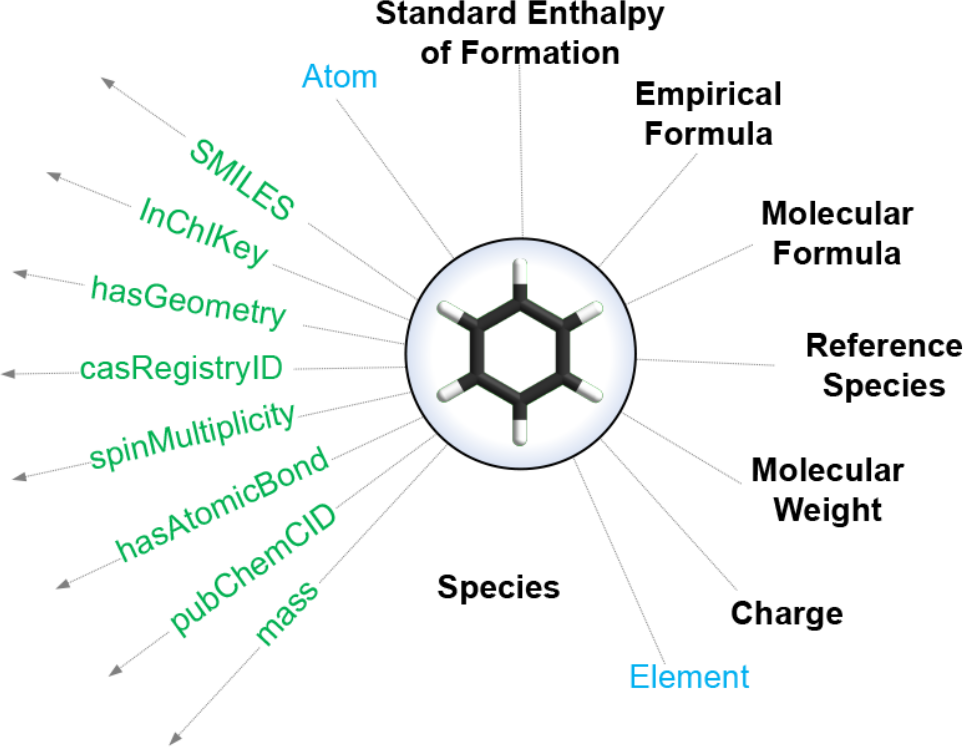
\includegraphics[height=2.40in,width=3.25in,viewport=0 0 990 750,clip]{Key_OntoSpecies-and-external_concepts.png}
\caption{\tiny\textrm{Key OntoSpecies (black) and external (blue) concepts, along with a number of properties (green) used to describe chemical species in TWA KG. cite from\cite{ACR56-128_2023}}}%(与文献\cite{EPJB33-47_2003}图1对比)
\label{Fig:Key-OntoSpecies-and-external-concepts}
\end{figure}
}

\frame
{
	\frametitle{\textrm{Agent}:~化学-化工知识图谱的组织工具}
	\textrm{Agent}:~能够感知环境、进行决策和执行动作的智能处理软件
	\begin{itemize}
		\item \textrm{Agent}工作方式类似于人类代理:~能接收输入数据(如传感器信息、文本、图像等),通过分析和处理数据,理解环境和任务要求,并做出相应的决策和行动
		\item 应用场景广泛,如自动驾驶车辆、智能机器人、语音助手等
		\item \textrm{Agent}核心功能:~感知、推理和决策
			\begin{itemize}
				\item 感知:~通过传感器等方式获取环境信息的能力,例如通过摄像头获取图像或通过麦克风获取声音
				\item 推理:~基于获取的信息进行逻辑推理和分析的能力,以了解环境和任务需求
				\item 决策:~根据推理结果做出相应的决策,并执行相应的动作
			\end{itemize}
		\item 通过与环境的交互和反馈,\textrm{Agent}可以逐步改进性能和表现,实现好的任务执行能力\\
		\item \textrm{Agent}设计和训练,需要结合机器学习和人工智能技术,如强化学习、深度学习等
	\end{itemize}
}

\frame
{
	\frametitle{知识图谱组织示例}
\begin{figure}[h!]
\centering
\vskip -8pt
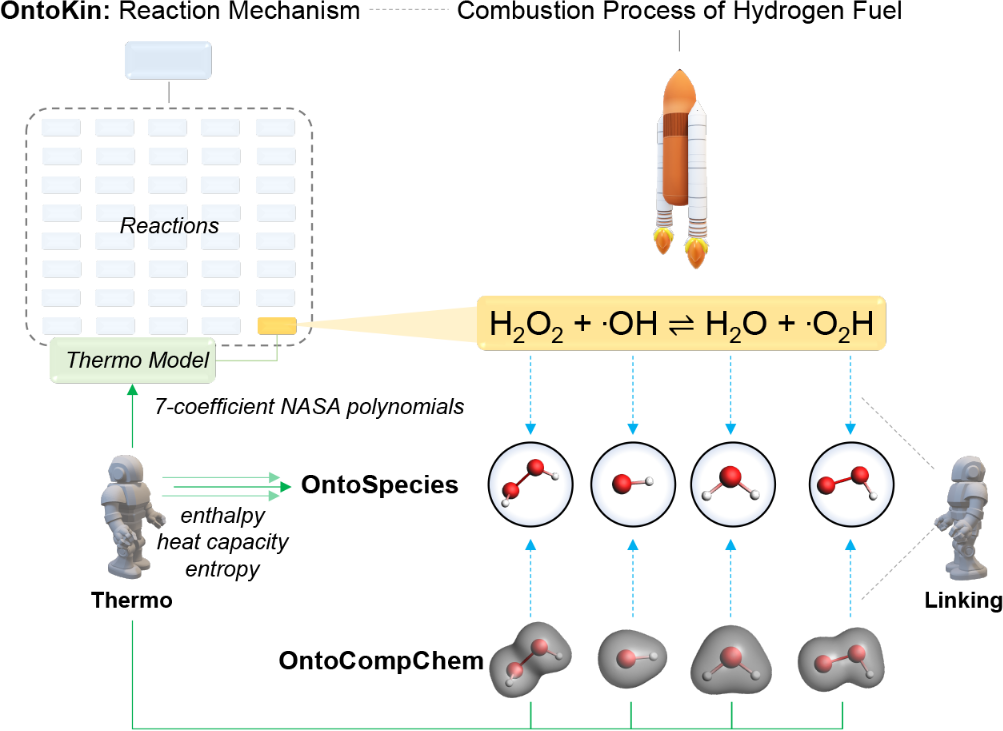
\includegraphics[height=2.70in,width=3.75in,viewport=0 0 1010 750,clip]{Automated-linking-between-OntoSepcies-Kin-CompChem.png}
\caption{\tiny\textrm{Automated linking between OntoSpecies, OntoKin and OntoCompChem. cite from\cite{ACR56-128_2023}}}%(与文献\cite{EPJB33-47_2003}图1对比)
\label{Fig:Automated-linking-between-OntoSpecies-Kin-CompChem}
\end{figure}
}

\frame
{
	\frametitle{知识图谱组织示例}
\begin{figure}[h!]
\centering
\vskip -8pt
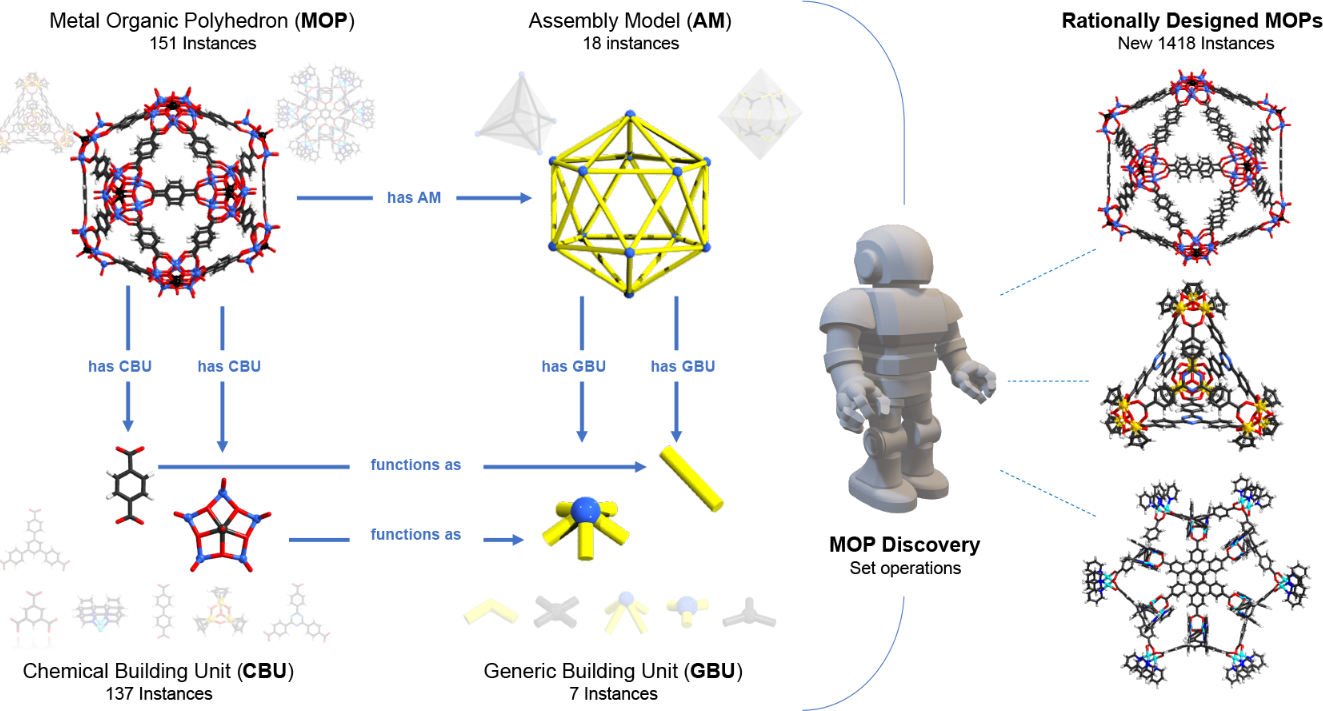
\includegraphics[height=2.20in,width=4.05in,viewport=0 0 1330 700,clip]{Key_concepts-in-OntoMOPs-and-designed-MOPs.png}
\caption{\tiny\textrm{Key concepts in OntoMOPs (left) and examples of newly rationally designed MOPs (right). cite from\cite{ACR56-128_2023}}}%(与文献\cite{EPJB33-47_2003}图1对比)
\label{Fig:OntoMOPs-MOPs}
\end{figure}
}

\frame
{
	\frametitle{化学-化工知识图谱建设的一些建议}
	化学-化工是一级学科,涉及知识点广泛,很难用一个知识\textrm{(Ontology)}简单地涵盖,建议参照上述化学-化工知识图谱方案,组织和构建化学-化工知识生态
	\begin{itemize}
		\item 以化学物种数据为核心知识
		\item 化学实验、化学计算知识的储备为桥梁
		\item 化学反应-实验、计算-物种的数据关联为目标
		\item 扩展各\textrm{Ontology}间数据分析、传递的\textrm{Agent}功能
		\item 通过\textrm{Ontology}-\textrm{Agent}数据迭代直至自洽
		\item 通过复杂计算和逻辑推理,产生新的物种属性描述或新的知识
	\end{itemize}
	\textcolor{magenta}{近期目标}:~在不远的将来,通过\textrm{Ontology}和\textrm{Agent}的复杂组合,有望改进和提升分子或材料的属性

\textcolor{magenta}{远期目标}:~建设完整的化学-化工知识的生态系统,通过化学知识空间的探索,有效地发现更多的新化学知识
}
%------------------------------------------------------------------------Reference----------------------------------------------------------------------------------------------
		\frame[allowframebreaks]
{
\begin{thebibliography}{99}
\frametitle{主要参考文献}
{\tiny
\bibitem{ACR56-128_2023}\textrm{A. Kondinski, J. Bai, S. Mosbach, J. Akroyd, and M. Kraft. \textit{Acc. Chem. Res.}, \textbf{56} (2023), 128}
}
\end{thebibliography}
%\nocite*{}
}
